\tocless \section{Giới thiệu}
LED 7 đoạn có 2 loại là Anode chung hoặc Kathode chung, ở dạng một LED 7 đoạn hoặc nhiều LED 7 đoạn ghép lại với nhau.

Gồm 7 LED đơn mắc với nhau theo thứ tự có thể hiển thị được các số từ $0 - 7$ (ngoài ra có thể có thêm dấu \verb|"."| để phân cách nhiều LED 7 đoạn với nhau), ta gọi các LED đơn này là $a$, $c$, $c$, $d$, $e$, $f$, $g$ (có thể có thêm $dp$).
\begin{figure}[!h]
\begin{center}
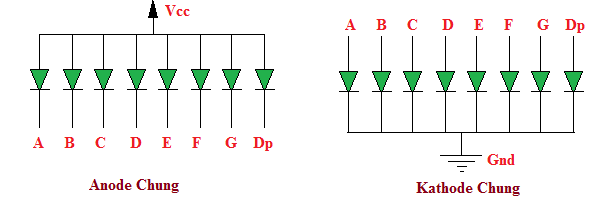
\includegraphics[scale=.6]{phu-luc/image/led-7-seg}
\end{center}
\caption{Sơ đồ chân của LED 7 đoạn}
\end{figure}
\begin{figure}[!h]
\begin{center}
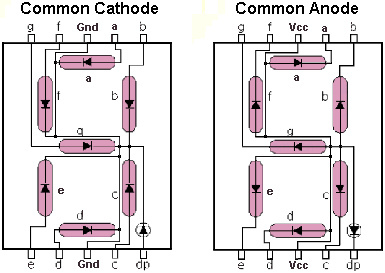
\includegraphics[scale=.4]{phu-luc/image/led-7-seg-anode-kathode}
\end{center}
\caption{Sơ đồ chân của LED 7 đoạn Anode hoặc Kathode chung ngoài thực tế}
\end{figure}
\tocless \subsection{LED 7 đoạn có Anode chung}
\begin{itemize}
\item Để hiển thị thanh LED nào, ta chỉ cần nối xuống chân $K$ của thanh LED đó xuống mass.
\item Sử dụng điện trở để hạn dòng cho LED.
\item Mã LED 7 đoạn Anode chung:
\begin{table}[!h]
\begin{center}
\begin{tabular}{|c|c|c|c|c|c|c|c|c|c|c|c|}\hline
\multirow{3}{.5cm}{\centering{Số}} & \multicolumn{8}{|c|}{Mã nhị phân} & \multicolumn{2}{|c|}{Mã HEX}\\ \cline{2-9}
& 7 & 6 & 5 & 4 & 3 & 2 & 1 & 0 & \multicolumn{2}{c|}{}\\ \cline{2-11}
& dp & g & f & e & d & c & b & a & dp & \\ \hline
0 & dp & 1 & 0 & 0 & 0 & 0 & 0 & 0 &  40 & C0\\ \hline
1 & dp & 1 & 1 & 1 & 1 & 0 & 0 & 1 &  79 & F9\\ \hline
2 & dp & 0 & 1 & 0 & 0 & 1 & 0 & 0 &  24 & A4\\ \hline
3 & dp & 0 & 1 & 1 & 0 & 0 & 0 & 0 &  30 & B0\\ \hline
4 & dp & 0 & 0 & 1 & 1 & 0 & 0 & 1 &  19 & 99\\ \hline
5 & dp & 0 & 0 & 1 & 0 & 0 & 1 & 0 &  12 & 92\\ \hline
6 & dp & 0 & 0 & 0 & 0 & 0 & 1 & 0 &  02 & 82\\ \hline
7 & dp & 1 & 1 & 1 & 1 & 0 & 0 & 0 &  78 & F8\\ \hline
8 & dp & 0 & 0 & 0 & 0 & 0 & 0 & 0 &  00 & 80\\ \hline
9 & dp & 0 & 0 & 1 & 0 & 0 & 0 & 0 &  10 & 90\\ \hline
A & dp & 0 & 0 & 0 & 1 & 0 & 0 & 0 &  08 & 88\\ \hline
B & dp & 0 & 0 & 0 & 0 & 0 & 1 & 1 &  03 & 83\\ \hline
C & dp & 1 & 0 & 0 & 0 & 1 & 1 & 0 &  46 & C6\\ \hline
D & dp & 0 & 1 & 0 & 0 & 0 & 0 & 1 &  21 & A1\\ \hline
E & dp & 0 & 0 & 0 & 0 & 1 & 1 & 0 &  06 & 86\\ \hline
F & dp & 0 & 0 & 0 & 1 & 1 & 1 & 0 &  0E & 8E\\ \hline
\end{tabular}
\end{center}
\caption{Mã LED 7 đoạn Anode chung}\label{Fig:led-7-seg-anode}
\end{table}
\end{itemize}
\tocless \subsection{LED 7 đoạn có Kathode chung}
\begin{itemize}
\item Để hiển thị thanh LED nào, ta chỉ cần nối xuống chân $A$ của thanh LED đó lên nguồn.
\item Sử dụng điện trở để hạn dòng cho LED.
\item Mã LED 7 đoạn Kathode chung:
\begin{table}[!h]
\begin{center}
\begin{longtable}{|c|c|c|c|c|c|c|c|c|c|c|c|}\hline
\multirow{3}{.5cm}{\centering{Số}} & \multicolumn{8}{|c|}{Mã nhị phân} & \multicolumn{2}{|c|}{Mã HEX}\\ \cline{2-9}
& 7 & 6 & 5 & 4 & 3 & 2 & 1 & 0 & \multicolumn{2}{c|}{}\\ \cline{2-11}
& dp & g & f & e & d & c & b & a & dp & \\ \hline
0 & dp & 0 & 1 & 1 & 1 & 1 & 1 & 1 &  BF & 3F\\ \hline
1 & dp & 0 & 0 & 0 & 0 & 1 & 1 & 0 &  86 & 06\\ \hline
2 & dp & 1 & 0 & 1 & 1 & 0 & 1 & 1 &  DB & 5B\\ \hline
3 & dp & 1 & 0 & 0 & 1 & 1 & 1 & 1 &  CF & 4F\\ \hline
4 & dp & 1 & 1 & 0 & 0 & 1 & 1 & 0 &  E6 & 66\\ \hline
5 & dp & 1 & 1 & 0 & 1 & 1 & 0 & 1 &  ED & 6D\\ \hline
6 & dp & 1 & 1 & 1 & 1 & 1 & 0 & 1 &  FD & 7D\\ \hline
7 & dp & 0 & 0 & 0 & 0 & 1 & 1 & 1 &  87 & 07\\ \hline
8 & dp & 1 & 1 & 1 & 1 & 1 & 1 & 1 &  FF & 7F\\ \hline
9 & dp & 1 & 1 & 0 & 1 & 1 & 1 & 1 &  EF & 6F\\ \hline
A & dp & 1 & 1 & 1 & 0 & 1 & 1 & 1 &  F7 & 77\\ \hline
B & dp & 1 & 1 & 1 & 1 & 1 & 0 & 0 &  FC & 7C\\ \hline
C & dp & 0 & 1 & 1 & 1 & 0 & 0 & 1 &  B9 & 39\\ \hline
D & dp & 1 & 0 & 1 & 1 & 1 & 1 & 0 &  DE & 5E\\ \hline
E & dp & 1 & 1 & 1 & 1 & 0 & 0 & 1 &  F9 & 79\\ \hline
F & dp & 1 & 1 & 1 & 0 & 0 & 0 & 1 &  F1 & 71\\ \hline
\end{longtable}
\end{center}
\caption{Mã LED 7 đoạn Kathode chung}\label{Fig:led-7-seg-kathode}
\end{table}
\end{itemize}
\tocless \subsection{IC ghi dịch 74HC595}
\begin{figure}[!h]
\begin{center}
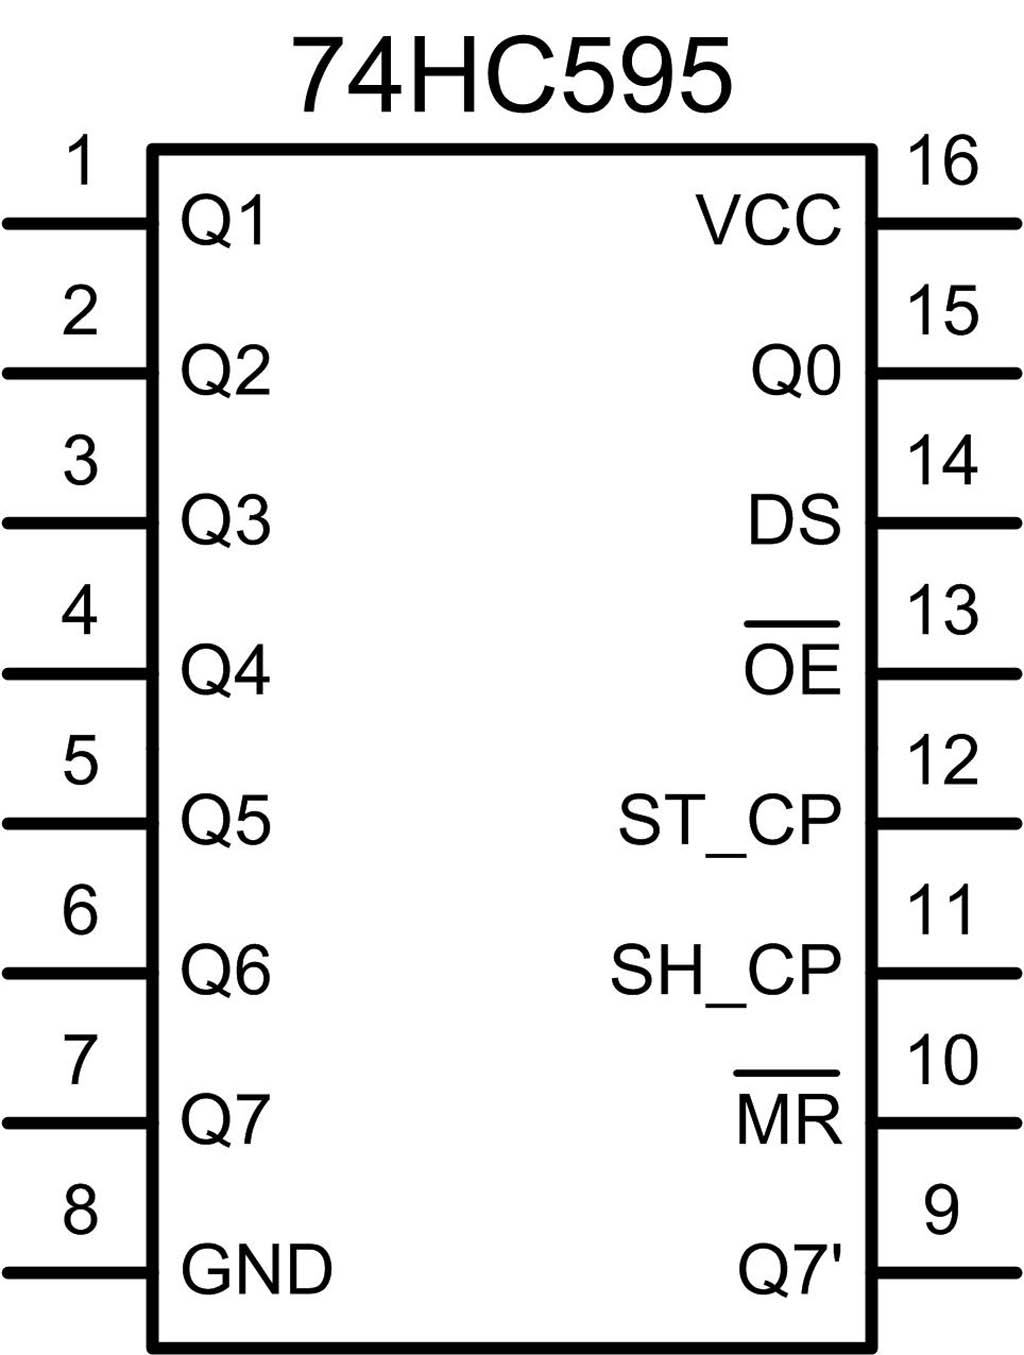
\includegraphics[scale=1.5]{phu-luc/image/74HC595}
\end{center}
\caption{Sơ đồ chân của IC ghi dịch 74HC595}\label{Fig:ngly-74hc595}
\end{figure}
Nguyên lý hoạt động của IC 74HC595:hình \ref{Fig:ngly-74hc595}
\begin{itemize}
\item Mô tả chức năng các chân:
\begin{itemize}
\item Input: chân $DS$: đầu vào dữ liệu nối tiếp. Tại mỗi thời điểm chỉ đưa vào 1 bit.
\item Output: từ chân $Q0 - Q7$. Xuất dữ liệu khi chân $\overline{OE}$ tích cực ở mức thấp và có một xung tích cực ở sườn âm tại chân chốt $ST\_CP$.
\item Output -- Enable: chân $\overline{OE}$: chân cho phép tích cực ở mức thấp. Khi nó ở mức cao thì không đầu ra nào được cho phép.
\item SQH: chân $Q7^\prime$: chân dữ liệu nối tiếp. Dùng để nối tiếp với IC 75HC595 khác, dữ liệu sẽ truyền cho IC tiếp theo khi nó đã nhận đủ được 8 bit.
\item Shift clock: chân $SH\_CP$: khi có một xung clock tích cực ở sườn dương thì 1 bit được dịch vào IC.
\item Latch clock: chân $ST\_CP$: xung chốt dữ liệu. Khi có một xung clock tích cực ở sườn dương thì cho phép xuất dữ liệu.
\item Chiều dịch bit: từ $Q0 \rightarrow Q7$.
\item Reset: chân $\overline{MR}$: chân này ở mức thấp thì dữ liệu sẽ bị xóa.
\end{itemize}
\item Nguyên lý hoạt động:
\begin{itemize}
\item Khi 1 bit được đưa vào chân $DS$, muốn đẩy bit này vào thanh ghi thì phải kích một xung vào chân $SH\_CP$ (xung sườn dương từ 0 lên 1). Làm như vậy, cho đến khi thanh ghi đủ 8 bit.
\item Dữ liệu 8 bit trong thanh ghi vẫn chưa thể xuất ra được, cần tạo một xung lên chân $ST\_CP$ (xung sườn dương từ 0 lên 1).
\item Khi dữ liệu quá 8 bit thì số bit còn dư sẽ đươc đưa đến chân $Q7^\prime$. Kết nối chân $Q7^\prime$ với chân $DS$ của IC tiếp theo để mở rộng chân.
\end{itemize}
\end{itemize}
\tocless \section{Phương pháp điều khiển}
Ta xét 2 phương pháp điều khiển: trực tiếp qua các chân \verb|I/O| và gián tiếp qua IC ghi dịch.
\begin{itemize}
\item Phương pháp điều khiển trực tiếp qua các chân \verb|I/O|:
\begin{itemize}
\item Ưu điểm: đơn giản.
\item Nhược điểm: tốn nhiều chân của vi điều khiển, không thể điều khiển số lượng lớn các LED 7 đoạn.
\end{itemize}
\item Phương pháp điều khiển gián tiếp qua IC ghi dịch:
\begin{itemize}
\item Ưu điểm: Dùng ít chân để điều khiển LED 7 đoạn (với IC 74HC595 chỉ dùng 3 chân của vi điều khiển có thể điều khiển được nhiều LED qua các IC ghi dịch này và có thể kết nối nhiều IC ghi dịch lại với nhau).
\item Khuyết điểm: phức tạp hơn phương pháp điều khển trực tiếp.
\end{itemize}
\end{itemize}
Khi sử dụng nhiều LED 7 đoạn được ghép chung với nhau, ta nên sử dụng phương pháp quét LED (bật tắt các LED một cách liên tục).
\tocless \section{Yêu cầu}
\paragraph{Yêu cầu 1}Sử dụng LED 7 đoạn đếm các số từ $0 - 9$ và từ $A-F$ bằng 2 phương pháp (điều khiển trực tiếp và điều khiển thông qua IC 74HC595).
\tocless \subsection{Phương pháp điều khiển trực tiếp}
\paragraph{Hướng giải quyết} Ta xuất giá trị của mã code ứng với loại LED 7 đoạn có Anode chung hay Kathode chung cho trong \textit{bảng \ref{Fig:led-7-seg-anode}} hoặc \textit{bảng \ref{Fig:led-7-seg-kathode}}.
\paragraph{Sơ đồ mạch}{~\\}
\begin{figure}[!h]
\begin{center}
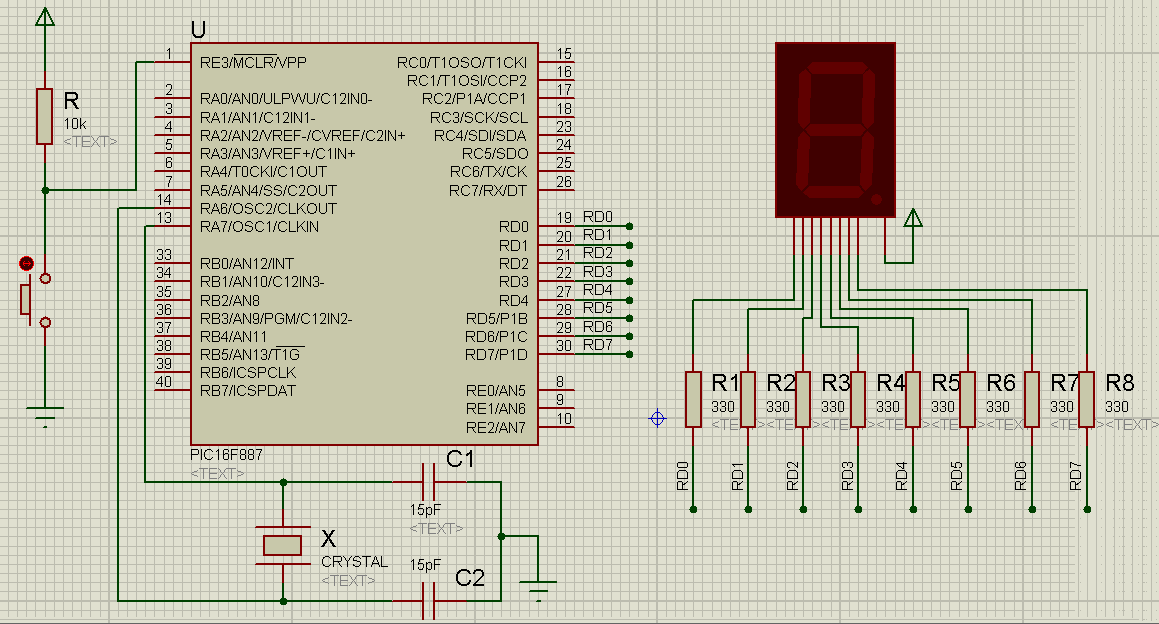
\includegraphics[scale=.5]{phu-luc/image/bai-2-phu-luc-led-7-seg}
\end{center}
\caption{Sơ đồ mạch điều khiển một LED 7 đoạn}
\end{figure}
\paragraph{Chương trình}{~\\}
\lstinputlisting[language=C]{BAI-2-PHU-LUC-LED-7-SEG-V1.C}
\newpage
\tocless \subsection{Phương pháp điều khiển thông qua IC ghi dịch 74HC595}
\paragraph{Sơ đồ mạch}{~\\}
\begin{figure}[!h]
\begin{center}
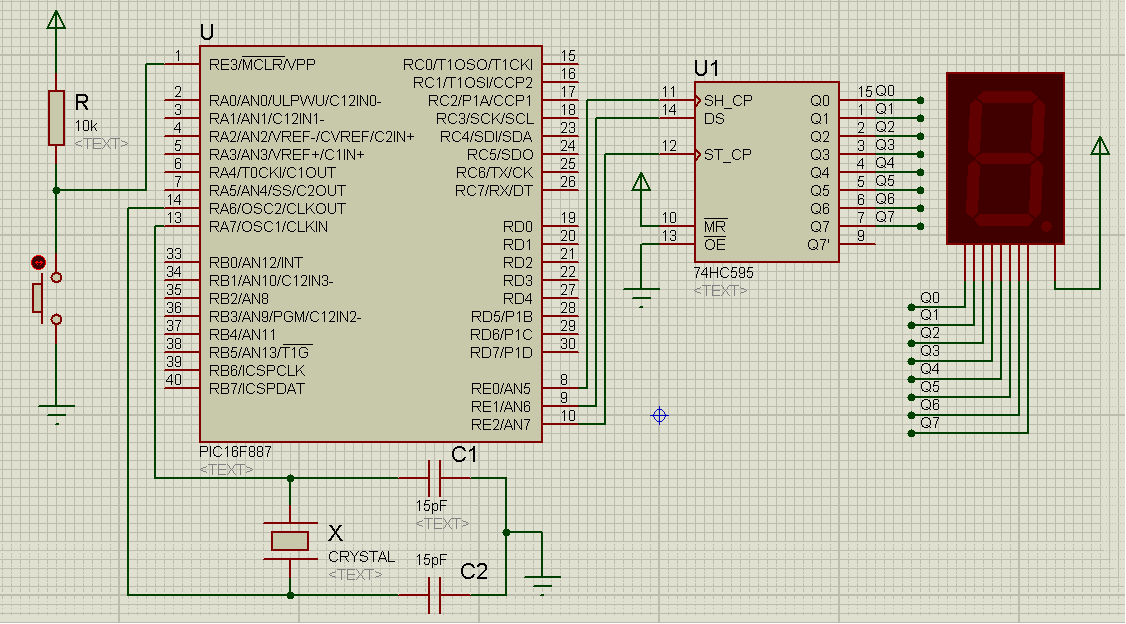
\includegraphics[scale=.5]{phu-luc/image/bai-2-phu-luc-led-7-seg-74hc595}
\end{center}
\caption{Sơ đồ mạch điều khiển một LED 7 đoạn qua IC 74HC595}
\end{figure}
\paragraph{Chương trình}{~\\}
\lstinputlisting[language=C]{BAI-2-PHU-LUC-LED-7-SEG-V2.C}
\paragraph{Yêu cầu 2}Sử dụng 4 LED 7 đoạn hiển thị các số từ $0 - 9999$ bằng 2 phương pháp (điều khiển trực tiếp bằng các chân và điều khiển thông qua IC 74HC595).
\tocless \subsection{Phương pháp quét LED -- Điều khiển trực tiếp qua các chân của vi điều khiển}
\paragraph{Sơ đồ mạch}{~\\}
\begin{figure}[!h]
\begin{center}
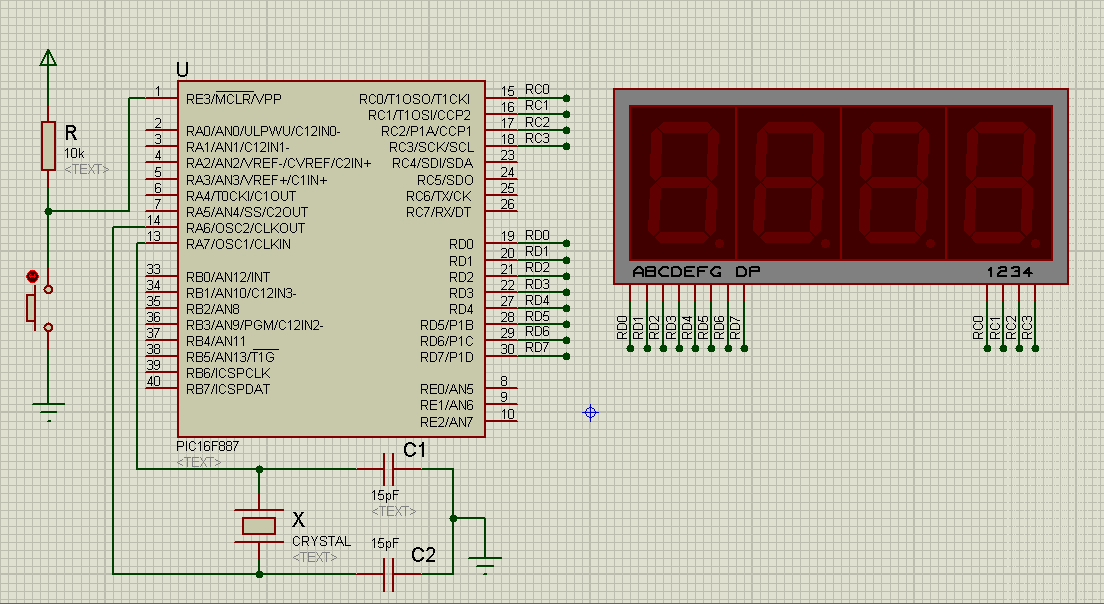
\includegraphics[scale=.5]{phu-luc/image/bai-2-phu-luc-4-led-7-seg}
\end{center}
\caption{Sơ đồ mạch điều khiển 4 LED 7 đoạn}
\end{figure}
\paragraph{Hướng giải quyết}
\begin{itemize}
\item Thường các LED loại này các thanh $a,b,c,d,e,f,g$ (có thể có $dp$) là chung với nhau, nó chỉ phân biệt nhau bằng số tự của LED 7 đoạn (mỗi LED 7 đoạn sẽ có một chân điều khiển).
\item Do đó, để hiển thị với nhiều LED 7 đoạn, ta dùng phương pháp quét LED: lặp lại quá trình bậc tắt các LED, khi đó sẽ đánh lừa được thị giác con người (do mắt người chỉ nhìn thấy được 24 điểm ảnh trên $1s$).
\item Với \textit{yêu cầu 2}, ta cần tách ra các chữ số riêng lẻ từ số ban đầu, rồi cho mỗi LED 7 đoạn hiển thị một số.
\end{itemize}
\paragraph{Chương trình}{~\\}
\lstinputlisting[language=C]{BAI-2-PHU-LUC-4-LED-7-SEG-V1.C}
\tocless \subsection{Phương pháp quét LED -- Điều khiển thông qua IC 74HC595}
\paragraph{Sơ đồ mạch}{~\\}
\begin{figure}[!h]
\begin{center}
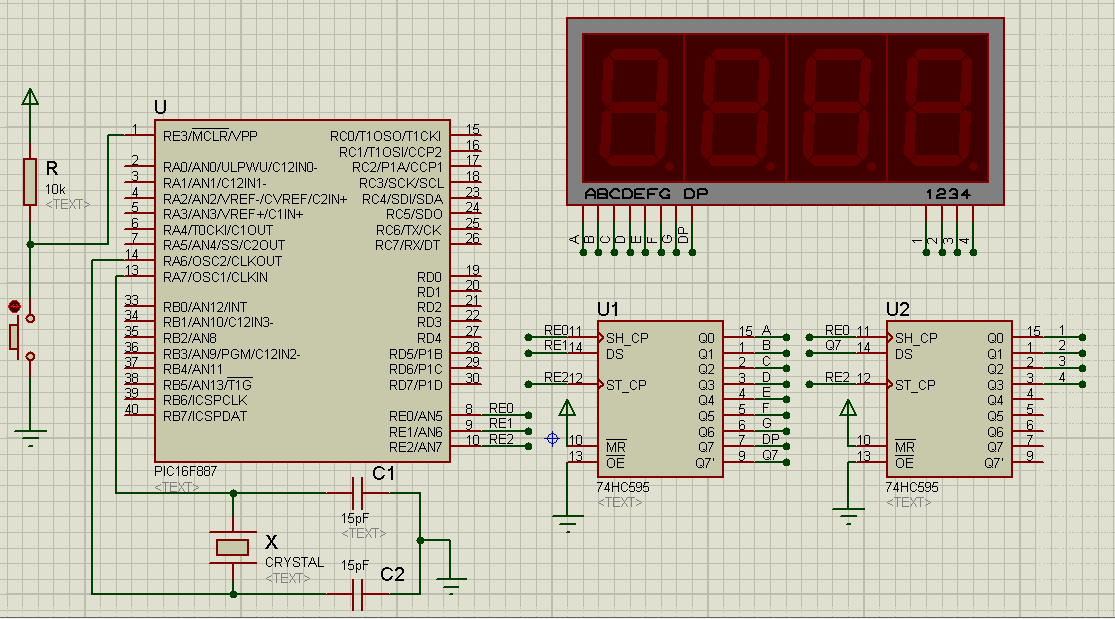
\includegraphics[scale=.5]{phu-luc/image/bai-2-phu-luc-4-led-7-seg-74hc595}
\end{center}
\caption{Sơ đồ mạch điều khiển 4 LED 7 đoạn qua IC 74HC595}
\end{figure}
\paragraph{Hướng giải quyết}
\begin{itemize}
\item Để tiết kiệm số chân điều khiển của vi điều khiển, ta dùng 2 IC 75HC595 để điều khiển 4 LED 7 đoạn.
\item Hoạt động theo nguyên tắc ngăn xếp: đưa vào sau sẽ lấy ra trước.
\item IC đầu tiên khi nhận đủ 8 bit, nếu tiếp tục gửi bit thì nó sẽ chuyển số bit dư sang chân $Q7^\prime$ để chuyển sang IC thứ 2.
\end{itemize}
\paragraph{Chương trình}{~\\}
\lstinputlisting[language=C]{BAI-2-PHU-LUC-4-LED-7-SEG-V2.C}
